\documentclass[a4paper]{article}
\usepackage[margin=1in]{geometry}
\usepackage[utf8]{inputenc}
\usepackage{amsmath}
\usepackage{graphicx}
\usepackage{hyperref}

\title{CSCI5525 Assignment 1 Answer}
\author{Daihui DOU\qquad dou00005@umn.edu\qquad 5514178 }

\begin{document}

\maketitle

\section{Problem 1}
(1) Let $\frac{\partial E[l(f(x),y)]}{\partial f(x)} = 0$, then
\begin{align*}
    \int_{y}(f(x)-y)p(y|x)p(x)\mathrm{d}y &=0 \\
    \int_{y}f(x)p(y|x)p(x)\mathrm{d}y &= \int_{y}yp(y|x)p(x)\mathrm{d}y
\end{align*}
Since $f(x)$ and $p(x)$ is independent of y, and $\int_{y}p(y|x)\mathrm{d}y = 1$,
\begin{align*}
    f(x)p(x)\int_{y}p(y|x)\mathrm{d}y &=  p(x)\int_{y}yp(y|x)\mathrm{d}y\\
    f(x) &= \int_{y}yp(y|x)\mathrm{d}y\\
     &= E[y|x]
\end{align*}
Thus the optimal $f(x)$ is $E[y|x]$, where $E[y|x]=\int_{y}yp(y|x)\mathrm{d}y.$\\
\\
(2) Let $\frac{\partial E[l(f(x),y)]}{\partial f(x)} = 0$, then
\begin{align*}
    \int \mathop{\rm sgn}(f(x)-y) p(y|x)p(x)\mathrm{d}y &= 0\\
    \int_{-\infty}^{f(x)} p(y|x)p(x) &= \int_{f(x)}^{\infty} p(y|x)p(x)
\end{align*}
which means the optimal $f(x)$ is the median of the distribution of y, i.e., $p(y\leq f(x)|x) = 0.5$.

\section{Problem 2}
The expectation for y is given by:
$$E[y]=\sum_{i=1:M}\int_{x\in \mathcal{R}_{i}}p(y_{i},x)\mathrm{d}x $$
The error rate for class $y=C_{j}$ equals to the rate that x is in $\mathcal{R}_{k}$ where $k\neq j$. Thus
\begin{align*}
    err[y=C_{j}]&=\sum_{i=1:M,i\neq j}\int_{x\in \mathcal{R}_{i}}p(y_{i},x)\mathrm{d}x \\
            &=\sum_{i=1:M,i\neq j}\int_{x\in \mathcal{R}_{i}}p(C_{j}|x)p(x)\mathrm{d}x \\
            &=\sum_{i=1:M}\int_{x\in \mathcal{R}_{i}}p(C_{j}|x)p(x)\mathrm{d}x-\int_{x\in \mathcal{R}_{j}}p(C_{j}|x)p(x)\mathrm{d}x
\end{align*}
Proved.
\section{Problem 3}
\subsection{(a)}
First modify the target T of boston dataset so that $p(y=0) = 0.5$ and $p(y=1) = 0.5$. And then Fisher's linear discriminant analysis (LDA) is applied to project boston dataset to 1 dimension. \\
Within-class covariance $S_{w}$ is given by:
$$S_{w} = \sum_{\mathbf{x}_{n}\in C_{1}} (\mathbf{x}_{n}-\mathbf{m}_{1})(x_{n}-\mathbf{m}_{1})^{T} + \sum_{\mathbf{x}_{n}\in C_{2}} (\mathbf{x}_{n}-\mathbf{m}_{2})(\mathbf{x}_{n}-\mathbf{m}_{2})^{T}$$
where $m_{i}$ is mean of class i, and weight vector $\mathbf{w}$ is given by:
$$\mathbf{w} \propto S_{w}^{-1}(\mathbf{m}_{2}-\mathbf{m}_{1})$$
and the projected data $f(x) = \mathbf{w}^{T}\mathbf{x}$. \\
The results of projected training data and test data of 10 cross-validation are below. Noted that LDA generally separated the two classes.\\
\\
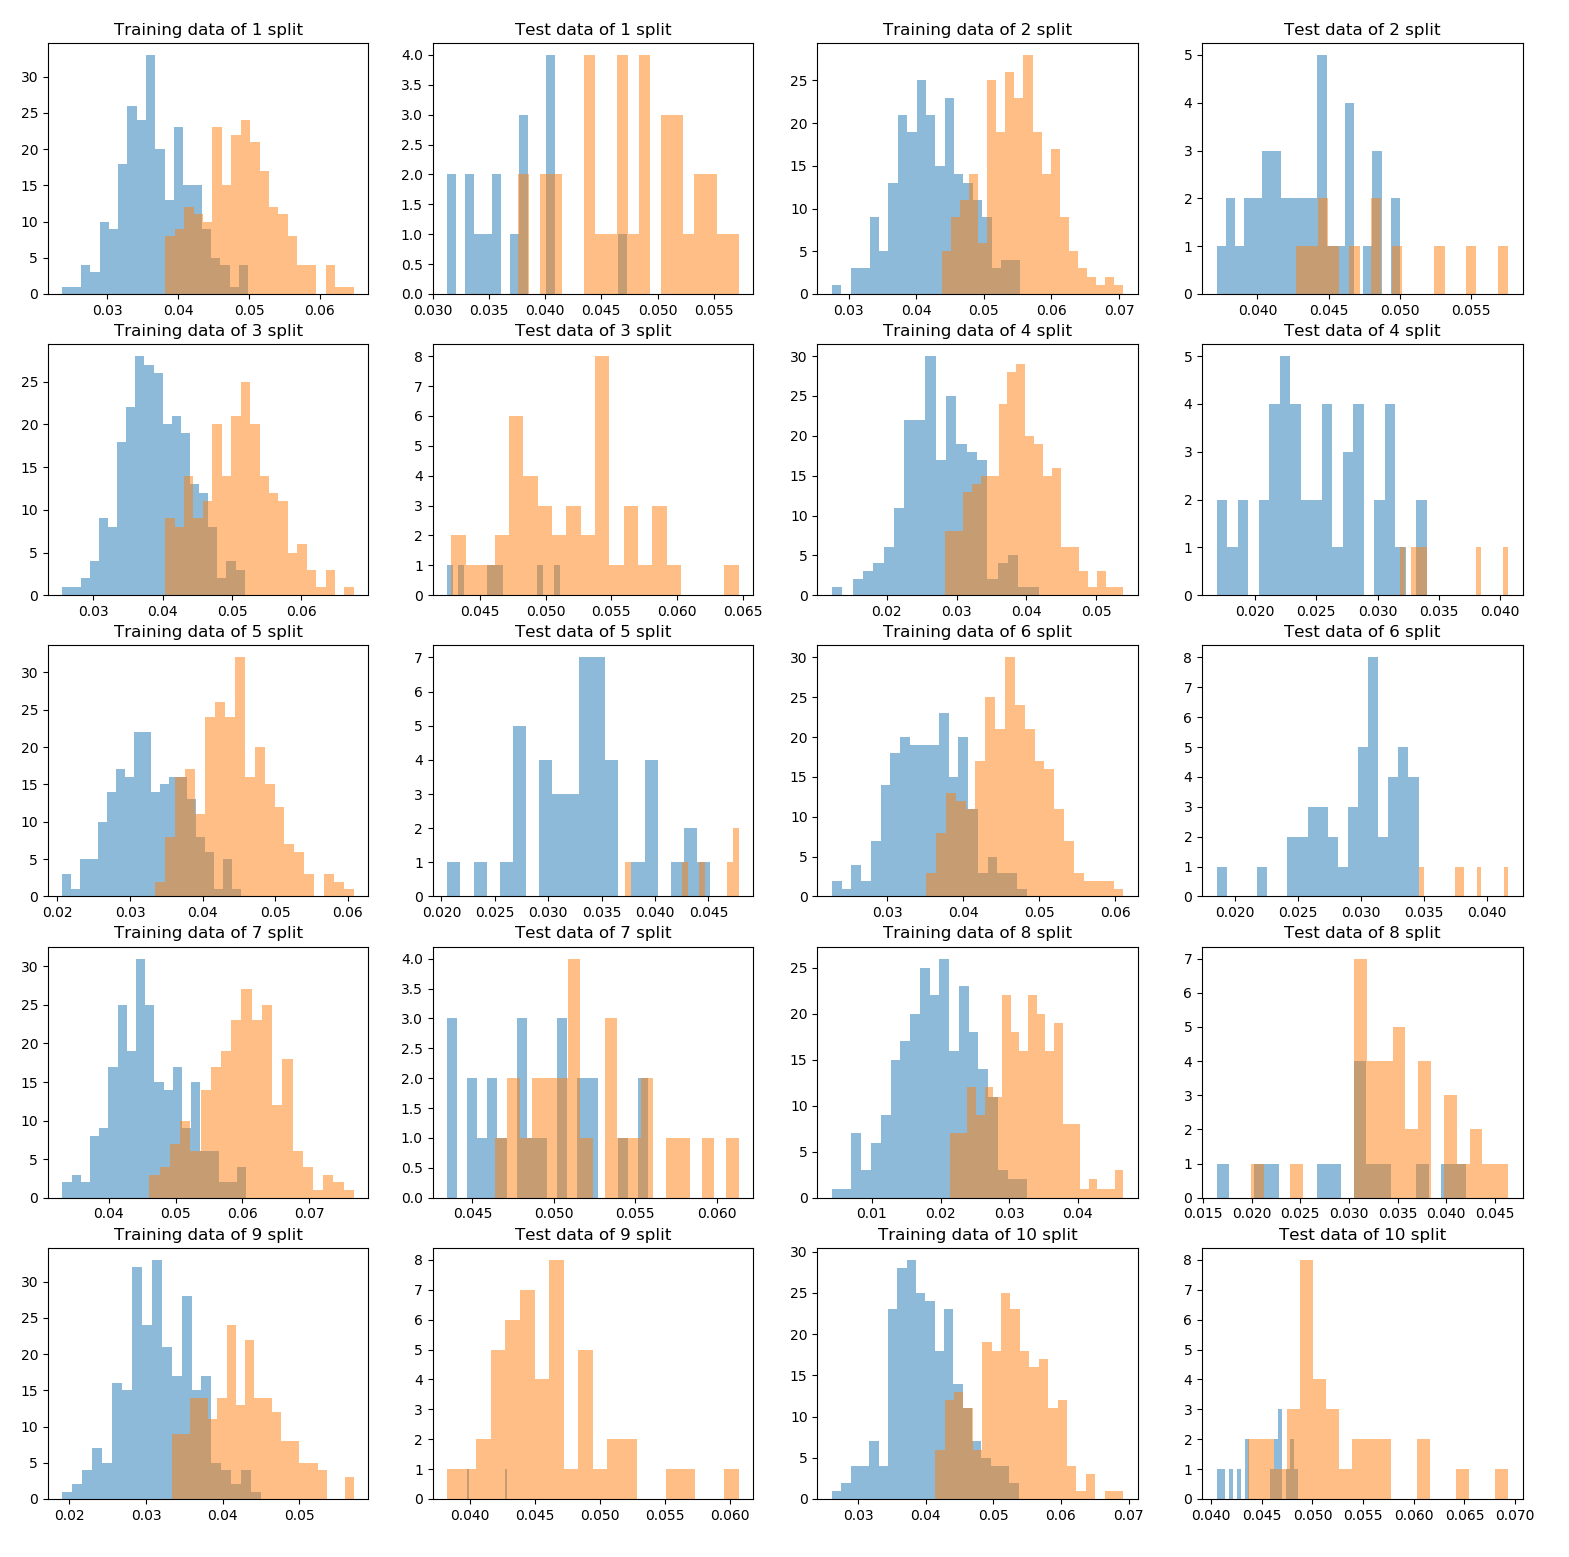
\includegraphics[width=\textwidth]{q3a.png}
\subsection{(b)}
No, since boston dataset has two classes after modification and LDA can project datasets to a maximum of $K-1$ dimensions, where $K$ is the number of classes.\\
This is because the maximum rank of between-class covariance $S_{b}$ is K-1, and thus for $S_{w}^{-1}S_{b}$ there are at most $K-1$ eigenvalues and corresponding $K-1$ eigenvectors. The subspace dimension of the projected data is given by the eigenvectors, which is at most $K-1$.
\subsection{(c)}
Between-class and within-class covariance $S_{w}$ is given by:
\begin{align*}
    S_{b} &= \sum_{i=1}^{K}N_{i}(\mathbf{m}_{i}-\mathbf{m})(\mathbf{m}_{i}-\mathbf{m})^{T}\\
    S_{w} &= \sum_{i=1}^{K}\sum_{x_{n}\in C_{i}}(\mathbf{x}_{n}-\mathbf{m}_{i})(x_{n}-\mathbf{m}_{i})^{T}
\end{align*}
where $K$ is the number of classes, $N_{i}$ is the number of instances in class i, $m_{i}$ is mean of class i.\\
The weight vector $\mathbf{w}$ is given by the top 2 eigenvectors of $S_{w}^{-1}S_{b}$ by the largest magnitude, and the projected data $f(x) = \mathbf{w}^{T}\mathbf{x}$. \\
The results of projected training data and test data of 10 cross-validation are below.\\
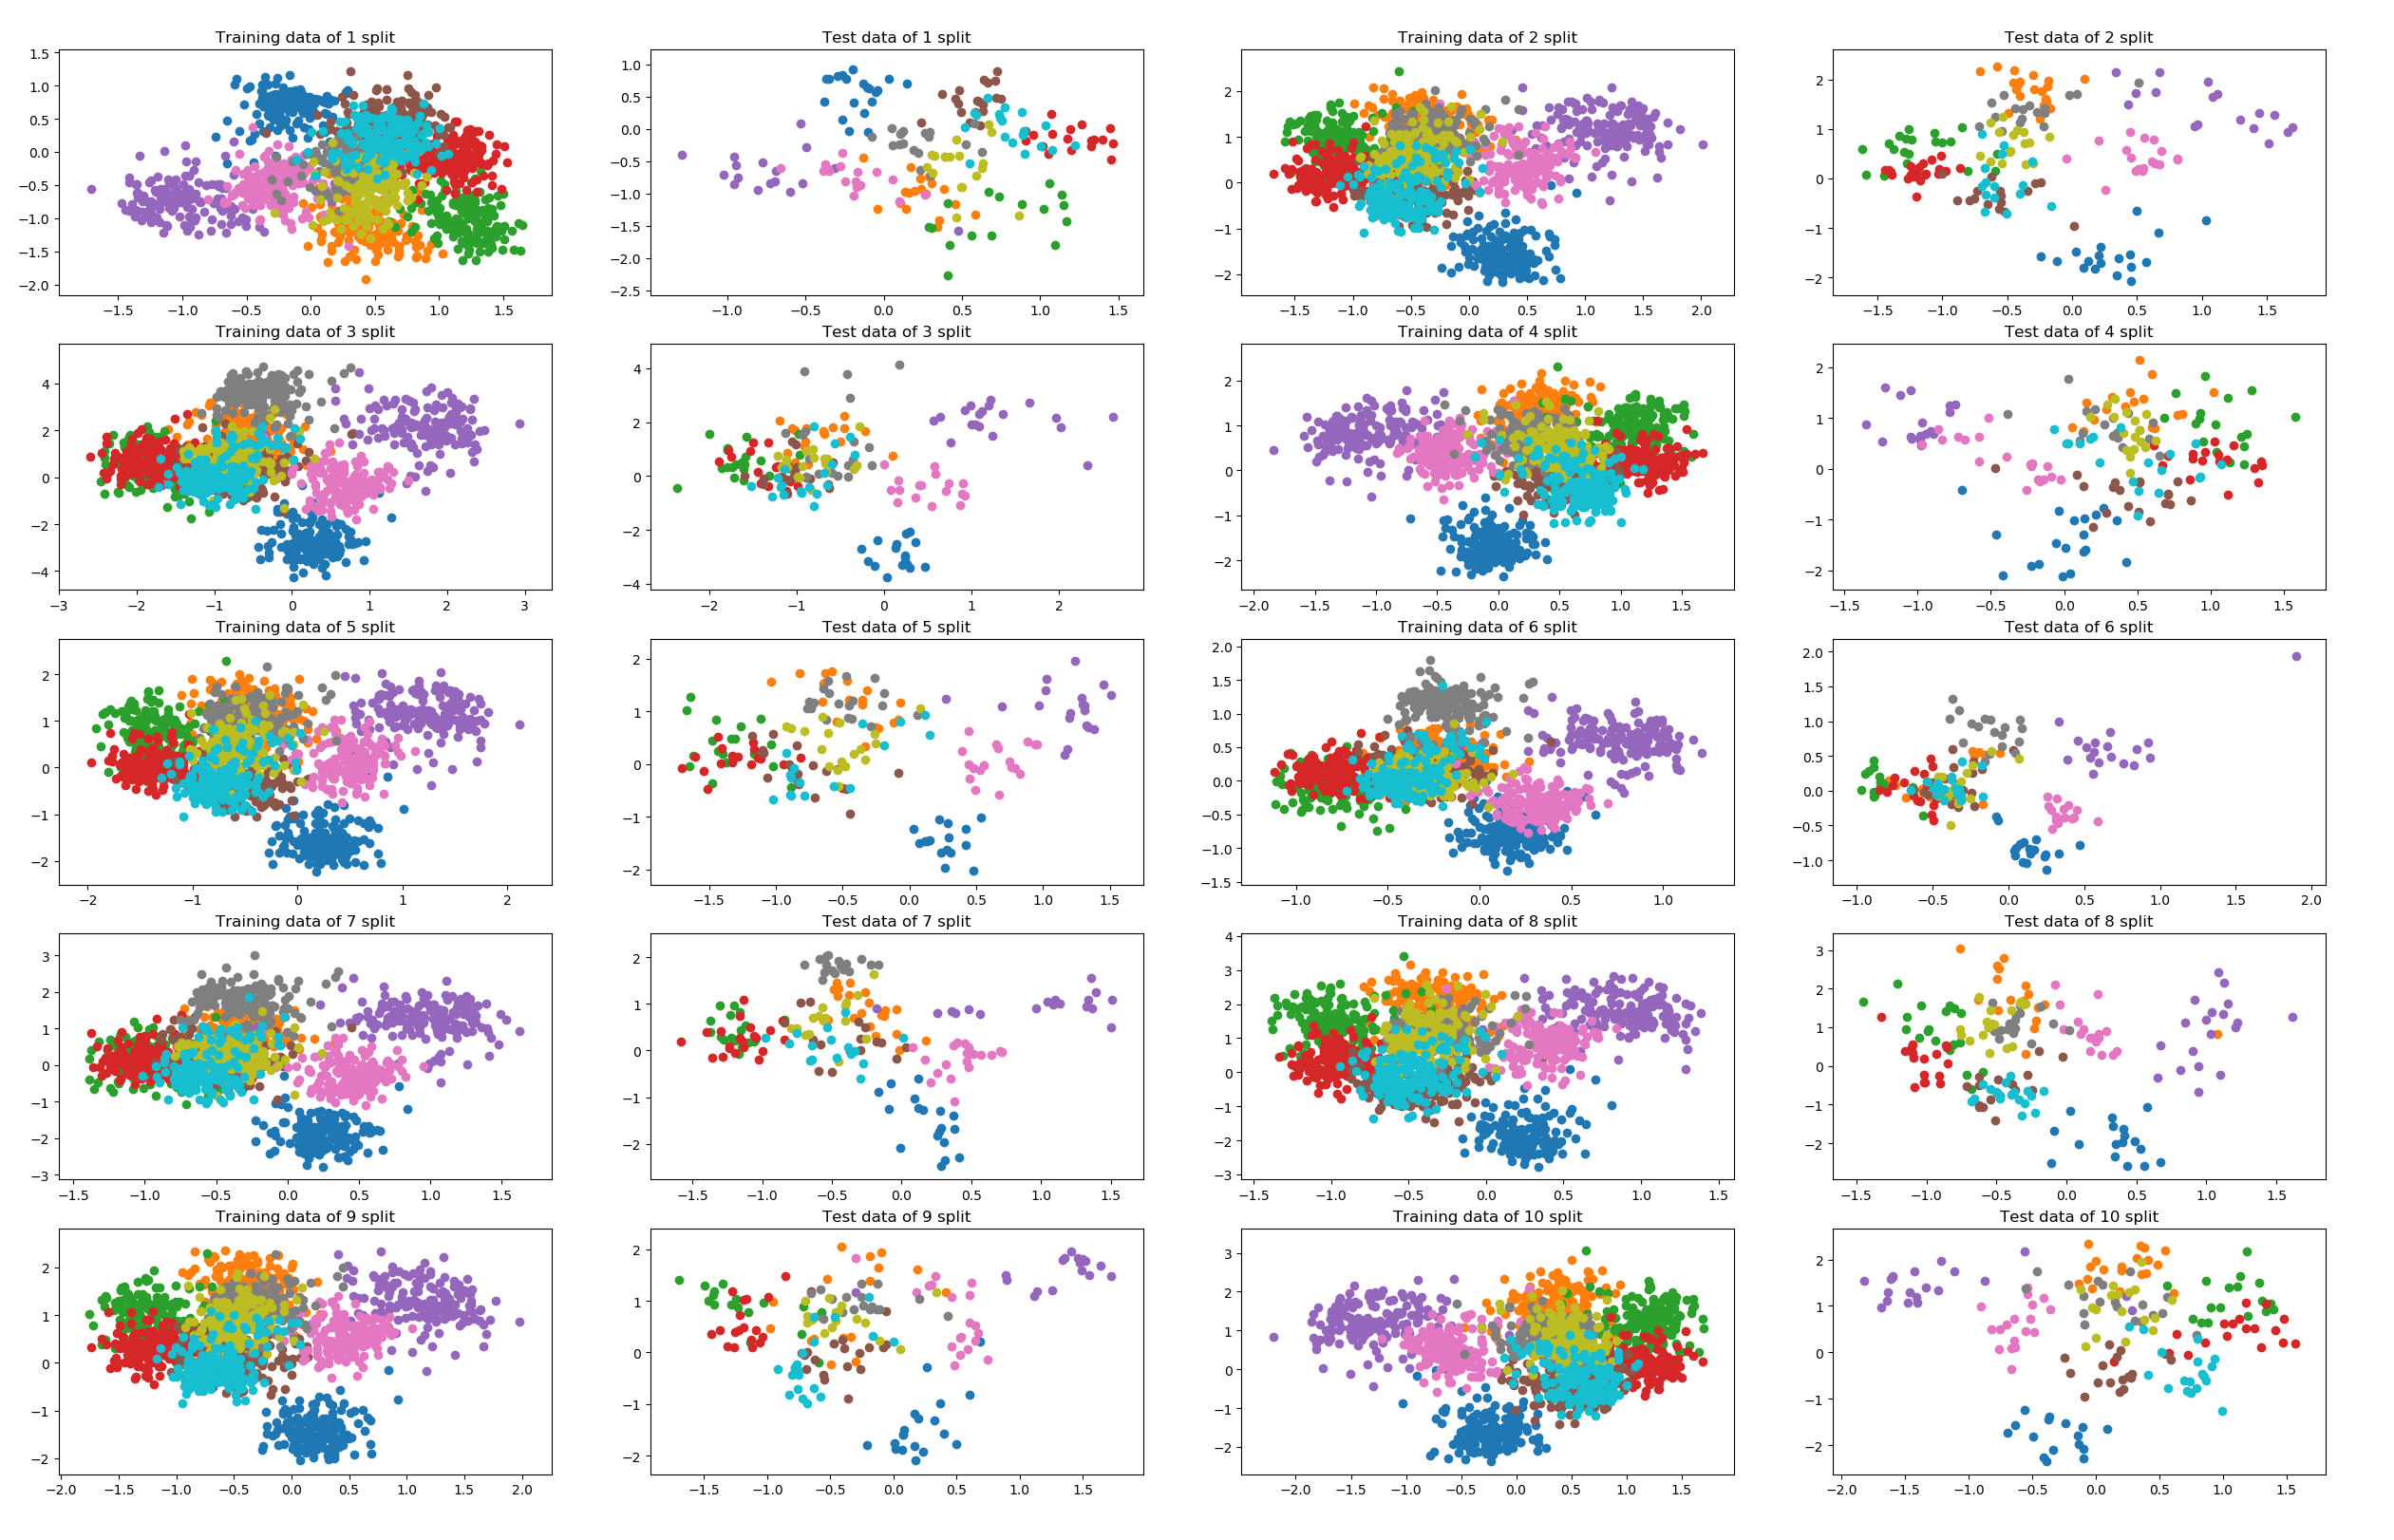
\includegraphics[width=\textwidth]{q3c.png}\\
The testing error followed by Gaussian generative modeling is bellow\\
\includegraphics[width=0.5\textwidth]{q3c_err.jpg}
\section{Problem 4}
\subsection{(a) Logistic regression (LR)}
Logistic regression is a discriminative model, and the class posteriors are given by:\\
$$p(C_{k}|\mathbf{x})=\frac{\exp(a_{k})}{\Sigma_{j}\exp(a_{j})}$$\\
where $a_{k}=\mathbf{w}_{k}^T\mathbf{x}$. Then the likelihood is given by:\\
$$p(\mathbf{y}|\mathbf{w}_{1},\dots,\mathbf{w}_{k}) = \prod_{n=1}^N\prod_{k=1}^K p(C_{k}|\mathbf{x}_{n})^{y_{nk}} = \prod_{n=1}^N\prod_{k=1}^K \pi_{nk}^{y_{nk}}$$\\
The optimization problem of $\mathbf{w}$ is solved by Iteratively Reweighted Least Squares (IRLS). Here the multi-class problem is treated as one-versus-the-rest problem. The update of $\mathbf{w}$ is then given by:\\
\begin{align*}
    \mathbf{w}^{new} &= \mathbf{w}^{old}-H^{-1}(\mathbf{w}^{old})\nabla E(\mathbf{w}^{old})\\
    &= (X^{T}RX)^{-1}X^{T}R\mathbf{z}
\end{align*}
where $\mathbf{z}=X\mathbf{w}^{old}-R^{-1}(\pi-\mathbf{y})$, and $R$ is a diagonal matrix initialized with $r^{i}=1$, which is updated by\\
$$r_{i}=\frac{1}{\max(\delta, |y_{i}-X^{i}\mathbf{w}|)}$$\\
where $\delta$ is some small value.
\subsection{(b) Naive-Bayes with marginal Gaussian distributions (GNB)}
For K-class problem of Naive-Bayes, the posterior probability for class k:
$$p(C_{k}|\mathbf{x})=\frac{p(\mathbf{x}|C_{k})p(C_{k})}{p(\mathbf{x})}=\frac{\exp(a_{k})}{\Sigma_{j}^{K}\exp(a_{j})}$$\\
were $a_{k}$ is given by:\\
$$a_{k}=\log p(\mathbf{x}|C_{k})+\log p(C_{k})$$\\
And for marginal Gaussian distribution, $p(x_{i}|C_{k})$ is given by:\\
$$p(x_{i}|C_{k})=\mathcal{N}(\mu_{ik}, \sigma_{ik}^{2})$$
$$p(\mathbf{x}|C_{k})=\prod_{n=1}^D p(x_{i}|C_{k})=\frac{1}{(2\pi)^{D/2}(\Pi_{i=1}^{D}\sigma_{ik})}\\
\exp \big(-\sum_{i=1}^{D}\frac{(x_{i}-\mu_{ik})^{2}}{2\sigma_{ik}^{2}}\big)$$\\
where $\mu_{k}$ and $\sigma_{k}^{2}$ are means and stds of class $k$ of training data.\\
\\
The results of LR and GNB are printed below:\\
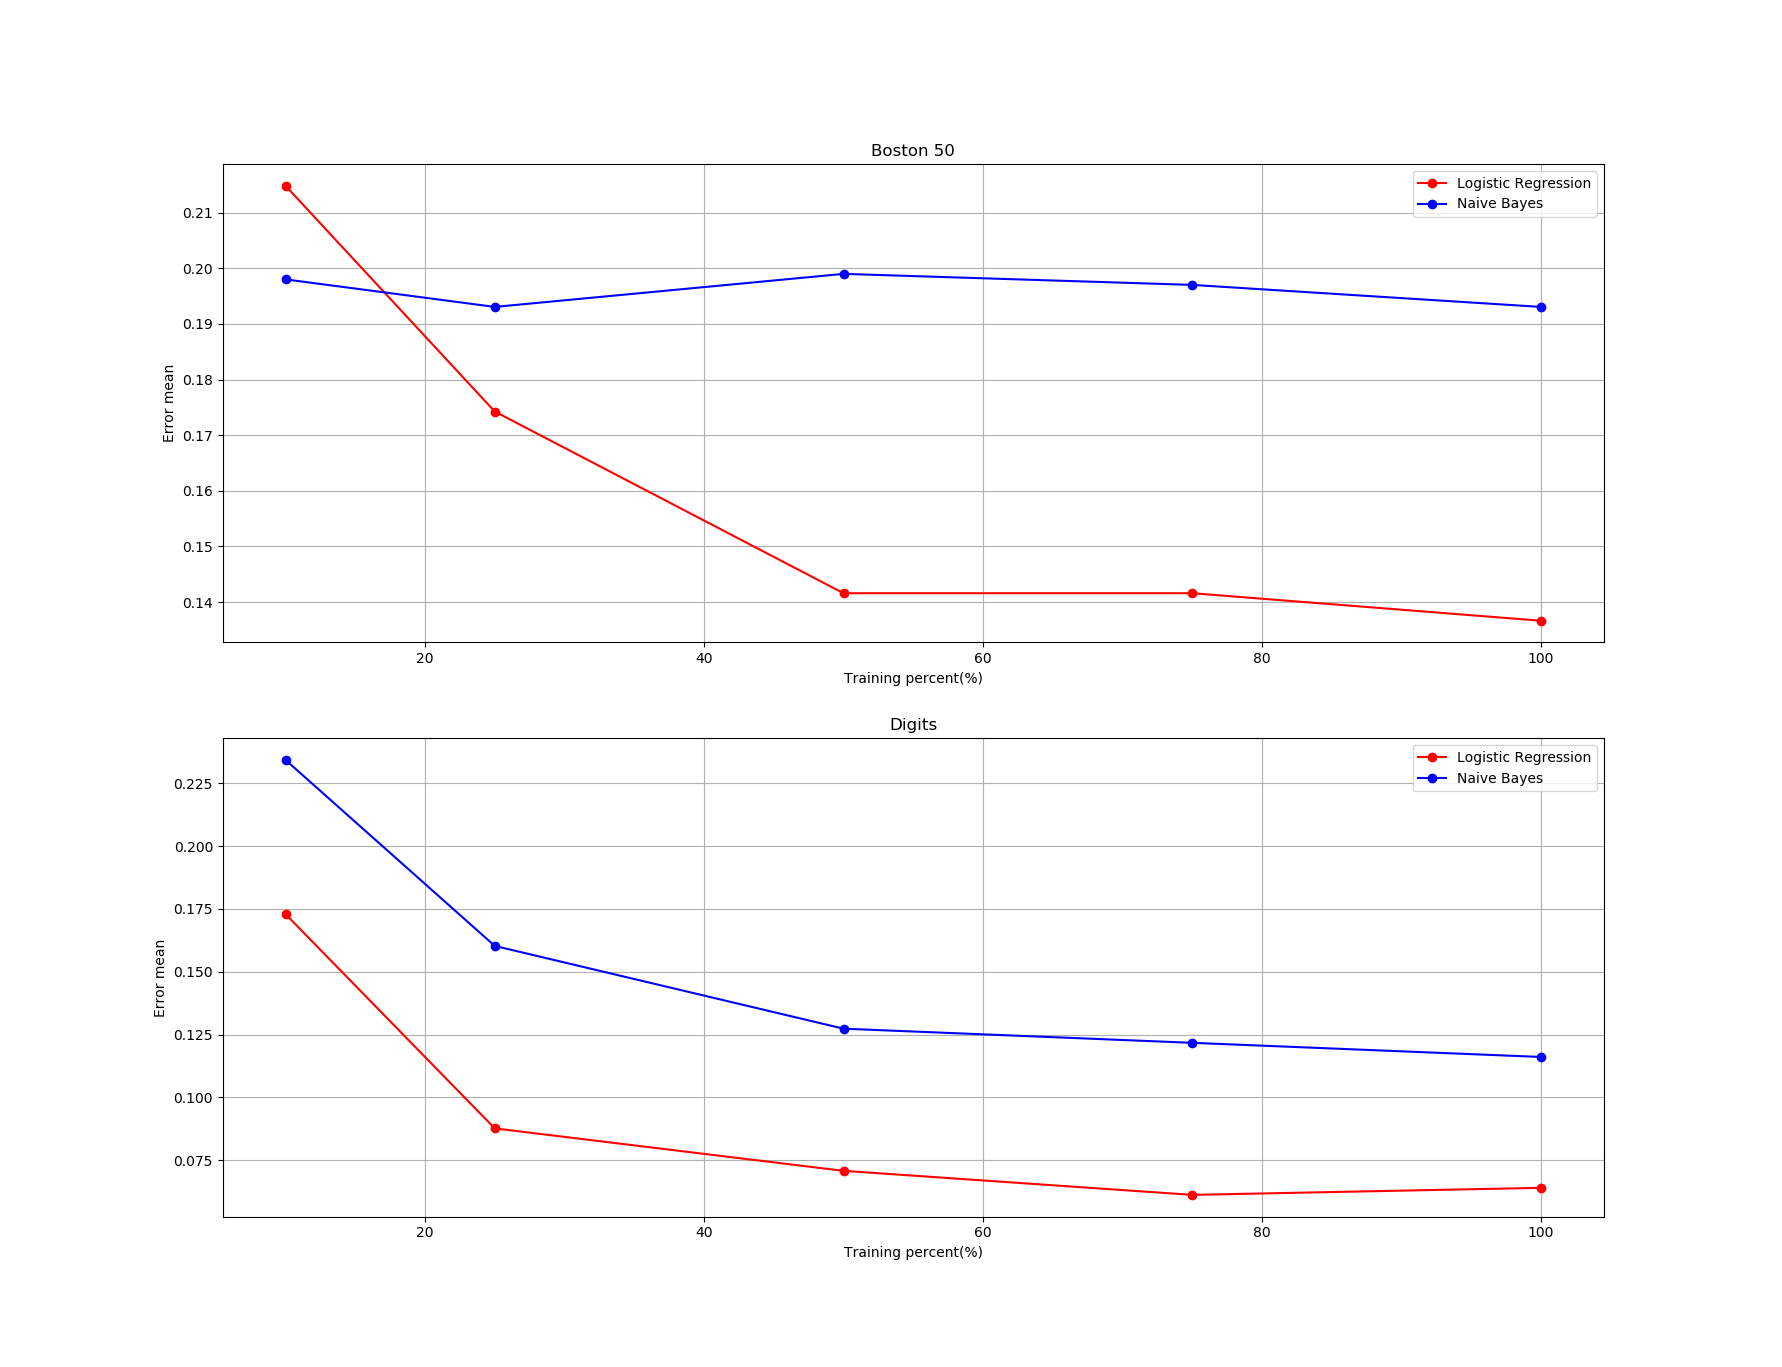
\includegraphics[width=\textwidth]{q4.png}\\
\end{document}